\documentclass[english]{cenarticle}
%----------------------------------------------------------------------------------------
%	PUBLISH INFO (not for authors)
%----------------------------------------------------------------------------------------
%
\issn{2179-460X}
%
\volume{44}
%
\eJournal{eXX}
%
\doi{https://doi.org/10.5902/2179460Xxxxxx}
%
\submitionDate{xx/xx/xx}
%
\approvalDate{xx/xx/xx}
%
\publishDate{xx/xx/xx}
%
\yearonfooter{xxxx}
%
%----------------------------------------------------------------------------------------
%	YOUR PACKAGES
%----------------------------------------------------------------------------------------
%
\usepackage{pgfplots}
\usepackage{caption}
\usepackage{graphicx}

\usepackage{amsmath,amsthm,amssymb,amsfonts}
\usepackage{siunitx}

\usepackage{booktabs}
\usepackage{multirow}
%
%----------------------------------------------------------------------------------------
%	YOUR CONFIGURATIONS
%----------------------------------------------------------------------------------------
%
\captionsetup{%
  font=footnotesize,
  labelfont=bf,
  singlelinecheck=false,
  tableposition=top,
  labelsep=endash,
  justification=raggedright,
  margin={0pt,0pt}
}

\sisetup{math-micro=\text{µ},text-micro=µ}
%
%----------------------------------------------------------------------------------------
%	YOUR NEW COMMANDS
%----------------------------------------------------------------------------------------
%
\renewcommand{\thefigure}{\arabic{figure}}
%----------------------------------------------------------------------------------------
%	PAPER INFO (for authors)
%----------------------------------------------------------------------------------------
%
\cenSection{Chemistry}
%
\englishTitle{Interference of Lightning and Thunder on Radioactivity: A Novel Approach in the air}
%
\portugueseTitle{Interferência de Raios e Trovões na Radioatividade: Uma Nova Abordagem no Ar}
%
\author{
  %\authorinfo[ORCID]{NAME}{AFFILIATION},
  \authorinfo[0000-0000-0000-0000]{Charles Babbage}{I},
  \authorinfo[]{Ada Lovelace}{II},
  \authorinfo[0000-0000-0000-0000]{Pierre Curie}{I},
  \authorinfo[0000-0000-0000-0000]{Marie Curie}{},
  \authorinfo[0000-0000-0000-0000]{Grace Hopper}{II},
  \authorinfo[0000-0000-0000-0000]{Santos Dumont}{},
  \authorinfo[]{Nikola Tesla}{},
  \authorinfo[0000-0000-0000-0000]{Galileu Galilei}{I},
  \authorinfo[0000-0000-0000-0000]{Charles Darwin}{I},
  \authorinfo[0000-0000-0000-0000]{Barbara McClintock}{}
}
%
\affil{ 
  \affiliation{I}{Brown University, USA}
  \affiliation{II}{University of Oxford, UK}
}

\shortHeaderTitle{Interference of Lightning and Thunder on Radioactivity: A Novel Approach ...}
\shortHeaderAuthors{Babbage{\it~et~al.}}
%
\portugueseAbstract{
Este artigo de pesquisa apresenta os resultados de um experimento conduzido por uma equipe de cientistas multidisciplinares, com o objetivo de estudar a interferência de raios e trovões na radioatividade. Utilizando o Electroplumbus nimbodetector, a equipe investigou as complexas interações entre raios, trovões e radioatividade, fornecendo insights fascinantes sobre esse fenômeno intrigante. A equipe coletou dados precisos e quantitativos sobre a intensidade dos raios e os níveis de radioatividade durante tempestades. Essas informações foram analisadas usando o algoritmo Foobar, permitindo a identificação de correlações e padrões. Além disso, a equipe realizou medições comparativas em áreas livres de atividade elétrica, servindo como grupo de controle para comparação de resultados. Essa abordagem meticulosa possibilitou uma análise mais precisa dos efeitos específicos da interferência dos raios na radioatividade. Os resultados obtidos revelam um aumento significativo nos níveis de radioatividade durante a ocorrência de raios e trovões, indicando uma clara influência desses fenômenos atmosféricos. Essa descoberta desafia suposições anteriores e contribui para o avanço do conhecimento sobre os efeitos da atividade elétrica na radioatividade. As implicações dessas descobertas são amplas e podem ter aplicações em várias áreas, incluindo segurança nuclear, proteção ambiental e até mesmo previsão de tempestades e seus efeitos potenciais.
}
%
\portugueseKeywords{raio, radioatividade, experimento aéreo, tempestade}
%
\englishAbstract{
This research paper presents the results of an experiment conducted by a team of multidisciplinary scientists, aimed at studying the interference of lightning and thunder on radioactivity. By utilizing the Electroplumbus nimbodetector, the team investigated the complex interactions between lightning, and radioactivity, providing fascinating insights into this intriguing phenomenon. The team collected accurate and quantitative data on the intensity of lightning, and levels of radioactivity during storms. This information was analyzed using the Foobar algorithm, allowing for the identification of correlations and patterns. Additionally, the team conducted comparative measurements in areas free from electrical activity, serving as a control group for result comparison. This meticulous approach enabled a more precise analysis of the specific effects of lightning interference on radioactivity. The obtained results reveal a significant increase in radioactivity levels during the occurrence of lightning and thunder, indicating a clear influence of these atmospheric phenomena. This discovery challenges previous assumptions and contributes to the advancement of knowledge regarding the effects of electrical activity on radioactivity. The implications of these findings are broad and can have applications in various fields, including nuclear safety, environmental protection, and even storm prediction and its potential effects.
}
%
\englishKeywords{lightning, radioactivity, airborne experiment, storm}
%
%----------------------------------------------------------------------------------------
\begin{document}
  \coverpage
%
\section{Experimental Setup}
\subsection{The 14-Bis flying vehicle}
The 14-Bis flying vehicle, an innovative experimental apparatus, features an open cockpit design that offers an unobstructed view for the driver during ascents into the skies to collect data within lightning storms. The vehicle is equipped with a two clicle kerosene fueled motor \citep{Torrens1992} that drives a large propeller, providing efficient propulsion for navigating through turbulent atmospheric conditions.\par
%
Its streamlined shape is optimized for aerodynamic efficiency, minimizing drag and turbulence to facilitate smooth movement through the air. The veicle incorporates pairs of rigid horizontal structures projecting from both sides, designed to provide stability and support during flight \citep{Wipo}, enabling the driver to maintain control even in the presence of strong winds and atmospheric disturbances.\par
%
Within the open cockpit, the driver securely straps into a harness, ready to embark on their mission into lightning storms. The propulsion system powered by the kerosene motor generates the necessary thrust for controlled ascent \citep{Torrens1992}, while the open design ensures an immersive experience for the driver, allowing them to observe and collect data in real-time.\par
%
With its purpose-driven design and reliable motor, the 14-Bis flying vehicle represents an instrumental tool for conducting data collection within lightning storms. The combination of an open cockpit, sturdy structural elements, and efficient propulsion system allows for precise maneuverability and enables researchers to gather valuable insights into the dynamics of these atmospheric phenomena.
%
\begin{figure}[!h]
  \caption{The 14-bis flying vehicle}
  \vspace{-3mm} 
  \begin{center}
    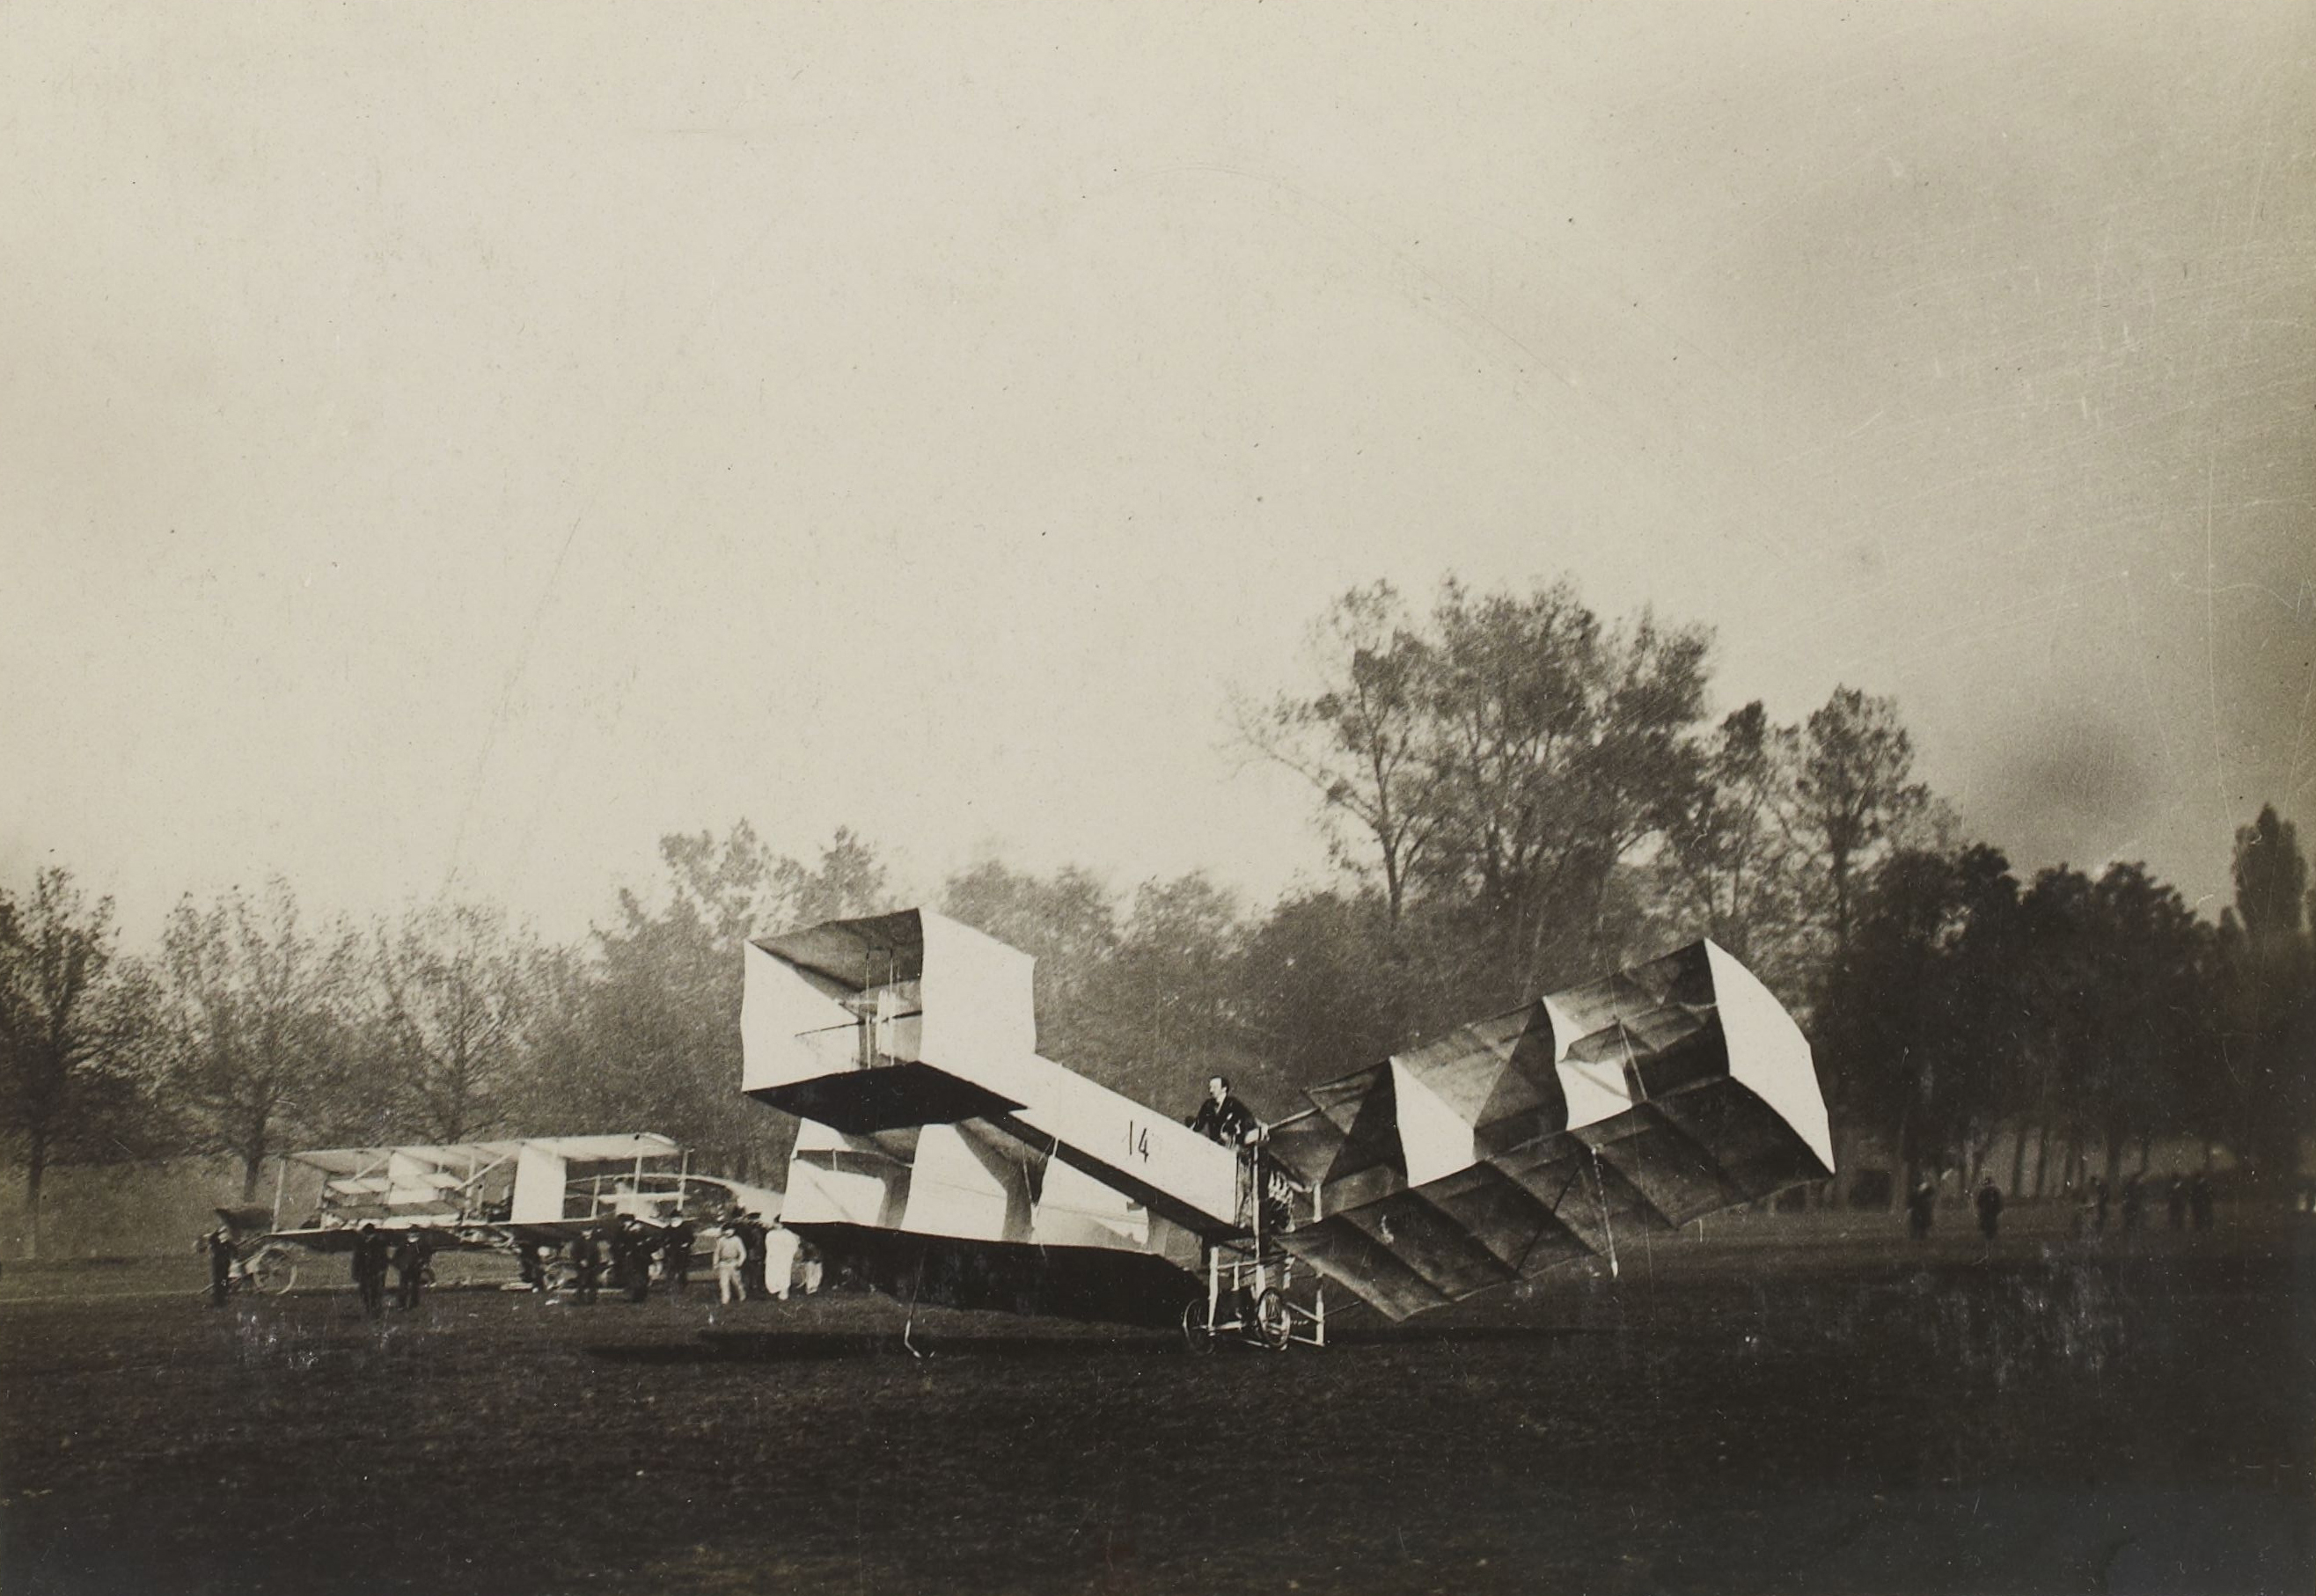
\includegraphics[width=0.55\textwidth, trim={0 0 0 0},clip]{images/14-bis.jpeg}
  \end{center}
  {\footnotesize
  Source: Biblioteca Digital Gallica, id btv1b8433366m, Public Domain, availiable on \citep{Beau1907}.\\
  Caption: The 14-bis in its final form, with octagonal-planform interplane ailerons.}
  \label{fig:triangle2}
\end{figure}

\subsection{Electroplumbus Nimbodetector}

Within the experimental setup, a key component is the 4th generation Electroplumbus Nimbodetector, a specialized device designed to collect data from sensors and measure radiation during lightning strikes. The core device of the Nimbodetector is a modified version of the Plumbus Combobulator, carefully adapted to precisely capture and analyze radiation levels at the exact moment of lightning occurrence.

The Electroplumbus Nimbodetector comprises two sensors strategically positioned on the front and rear of the 14-bis flying vehicle. These sensors, with a prism shape, are filled with an enriched Glowing Schleem substance specifically engineered to effectively gather data from lightning discharges. The Schleem material exhibits unique properties that enable accurate measurement of radiation within the immediate vicinity of lightning strikes.

To facilitate data transmission, the sensors are connected to the core device of the Electroplumbus Nimbodetector via electrical wires. This wired connection ensures reliable and swift data transfer, allowing for further analysis of radiation levels associated with lightning activity.

The inclusion of two sensors in the setup serves a crucial purpose: calculating the distance from the lightning source. By analyzing the time difference in data readings between the front and rear sensors, we can accurately estimate the distance traveled by the lightning strike.

\begin{figure}[!h]
  \newcommand\x{0.25}
  \caption{The 4th generation of the Electroplumbus Nimbodetector}
  \begin{center}
    \vspace{-3mm}
		\begin{minipage}[t]{\x\linewidth}
			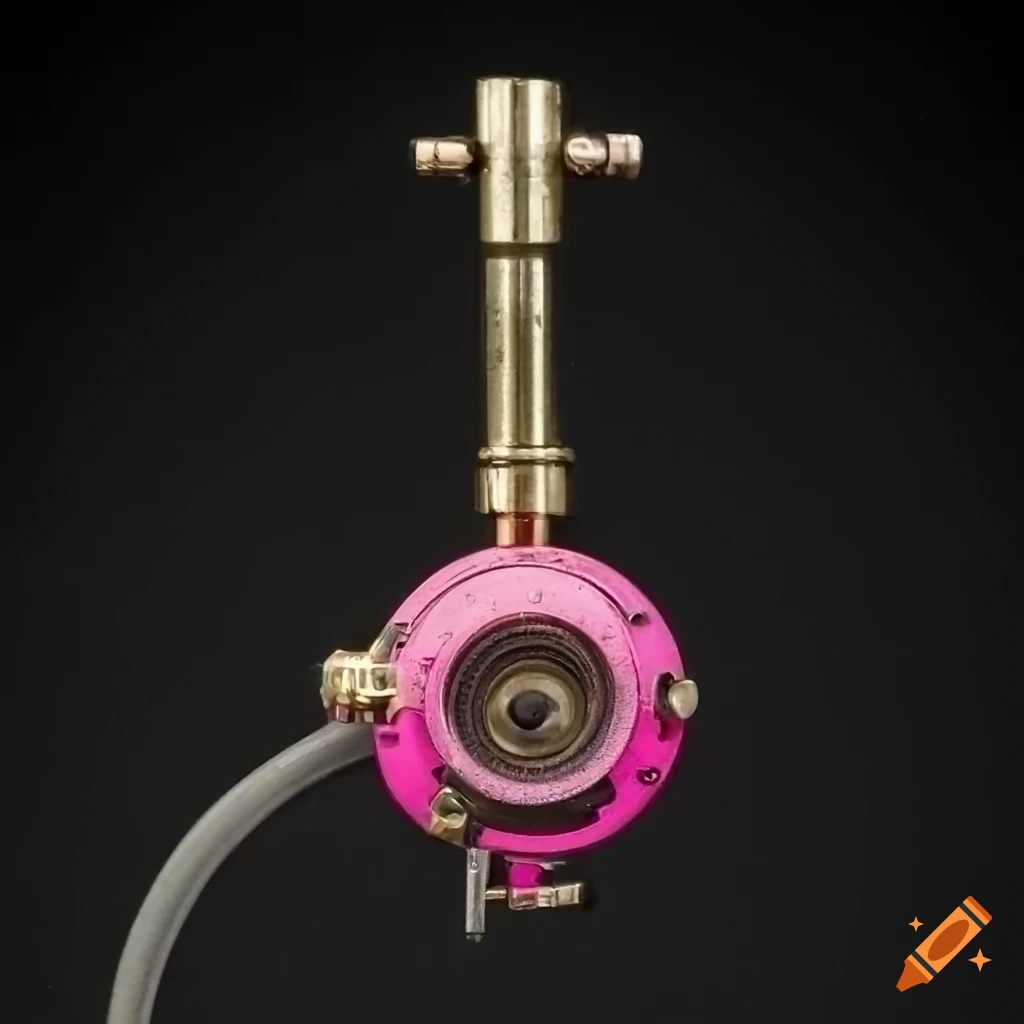
\includegraphics[width = \textwidth, trim={0 0.8cm 0 0.9cm},clip]{images/nimbodetector.png}	
      \captionsetup{justification=centering, font=footnotesize}
			\caption*{(a)}\label{fig:triangle2a}
		\end{minipage}
		\begin{minipage}[t]{\x\linewidth}
			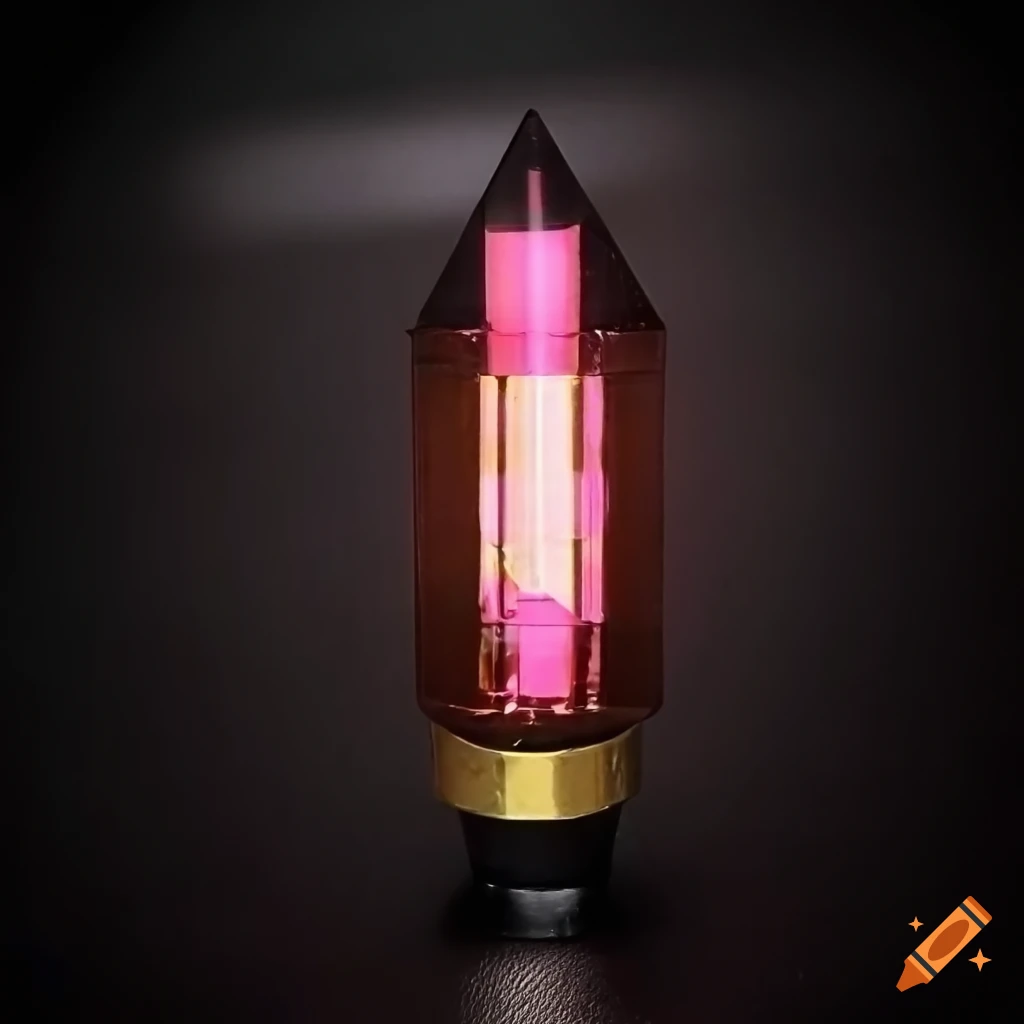
\includegraphics[width = \textwidth, trim={0 0.8cm 0 0.9cm},clip]{images/sensor.png}	
      \captionsetup{justification=centering, font=footnotesize}
			\caption*{(b)}\label{fig:triangle2b}
		\end{minipage}\\
  \end{center}%
  \vspace{-1mm}
  {\footnotesize
  Source: Craiyon website, see \citep{Craiyon}.\\
  Caption: The (a) figure displays the core of the device with the Plumbus Combobulator inside and (b) shows the lightning detector filled by enriched Glowing Schleem substance.\\
  }
	\label{fig:triangle2}
  \end{figure}\vspace{-9mm}
%
\subsection{Data Collection}

The data storage component of the Electroplumbus Nimbodetector is an essential element of its operational framework. This system employs a carefully engineered adaptation of the Plumbus Combobulator, which offers fault-tolerant characteristics and efficient data preservation.

At the core of the data storage mechanism is the utilization of punched paper, designed to withstand various environmental conditions. This robust material ensures the durability and integrity of the captured lightning data, even during adverse weather conditions such as rainfall. The waterproof nature of the paper safeguards the data from moisture, allowing for uninterrupted data collection.

The adapted Plumbus Combobulator employs a $\SI{0.47}{\micro\meter}$ needle, precisely marking the punched paper as the lightning data is processed. This needle-based mechanism creates a distinct pattern that represents the collected information. With each stroke, a tangible record of the lightning data is imprinted onto the punched paper.

The paper-based storage medium enables efficient and reliable data preservation. Each $\SI{100}{\milli\meter}$ segment of the punched paper corresponds to a substantial $\SI{1.2E6}{\byte}$ of information. This capacity ensures ample storage space for capturing an extensive volume of lightning data during experiments.

\section{Data Analysis}

\subsection{The Branzine}

According to Plumbus Combobulator manufacturer \citep{PlumbusManual}, the Branzine levels can cause Electroplumbus Nimbodetector malfunctions. Because that a preliminary exploratory flight was undertaken to examine the influence of altitude on Branzine levels, considering both air samples collected with and without rainfall.

During the flight, air samples were gathered at various altitudes to measure the concentration of Branzine, by using the Branzine detector\footnote{Digital Bz897U, available on $^{\circledR}$Airbone Laboratory Instrument Inc.}. The samples were divided into two groups: those collected during rainfall and those obtained under dry conditions. This differentiation aimed to explore any potential impact of precipitation on Branzine levels.


The collected data was send to the laboratory, and the results are summarized in the table below:

\begin{table}[!h]
\caption{Branzine levels}
\vspace{-6mm}
\footnotesize
\begin{center}
  \begin{tabular}{@{}lccc@{}}
  \toprule
                                         & altitude & \multicolumn{2}{c}{Branzine levels {$[ppm]$}} \\ \cmidrule(l){3-4} 
                                         & {$[m]$}  & on rain             & lack of rain            \\ \midrule
  \multirow{8}{*}{\rotatebox[origin=c]{90}{under the clouds} } 
                                         & $100 \pm 1$      & $0.005 \pm 0.001$   &     $0.006 \pm 0.001$  \\
                                         & $200 \pm 1$      & $1.265 \pm 0.001$   &     $1.260 \pm 0.001$  \\
                                         & $500 \pm 1$      & $40.1  \pm 0.01$    &      $40.2 \pm 0.01$   \\
                                         & $1000\pm 1$      & $392   \pm 5$       &      $395  \pm 5$      \\
                                         & $2000\pm 1$      & $609   \pm 5$       &      $607  \pm 5$      \\
                                         & $3000\pm 1$      & $2709  \pm 10$      &     $2701  \pm 10$     \\
                                         & $4000\pm 1$      & $12701 \pm 10$      &     $12699 \pm 10$     \\
                                         & $5000\pm 1$      & $100831 \pm 10$     &     $100827 \pm 10$    \\ \midrule
  \multirow{7}{*}{\rotatebox[origin=c]{90}{above the clouds} }
                                         & $6000\pm 1$       & $-$                &    $280190 \pm 10$                 \\
                                         & $6200\pm 1$       & $-$                &    $518914 \pm 100$                \\ 
                                         & $6400\pm 1$       & $-$                &    $819827 \pm 100$                \\ 
                                         & $6600\pm 1$       & $-$                &    $100827 \pm 100$                \\ 
                                         & $6800\pm 1$       & $-$                &    $1124225 \pm 1000$              \\ 
                                         & $7000\pm 1$       & $-$                &    $6131823 \pm 1000$              \\ 
                                         & $8000\pm 1$       & $-$                &    $9792921 \pm 1000$              \\ \bottomrule
  \end{tabular}\\[3mm]
\end{center}
Caption: The Branzine levels in relation to altitude, over the Atlantic Ocean (August, 1987).\\
\end{table}

Upon analyzing the data, it was observed that there is a increase in Branzine levels with increasing altitude. However, the rise remained below $0.2\%$, indicating an insignificant effect on the Plumbus performance. These findings align with prior research \citep{Gagaia1923}, which suggests that Branzine levels typically exhibit a notable increase of over $5\%$ in specific regions such as winter sections or the Bermuda Triangle ($32\%$).
\vfill

\pgfplotstableread{multiple_functions.dat}{\table}

\pgfplotsset{
  legend style = {font = \large}, % Adjust the font size and style as needed
  tick label style = {font = \Large}, % Adjust the font size as needed
  every axis label = {font = \Large}, % Adjust the font size as needed
}
 
\begin{center}
  \begin{tikzpicture}[scale=0.7][H]
\begin{axis}[
    xmin = 0, xmax = 10,
    ymin = 0, ymax = 1,
    xtick distance = 1,
    ytick distance = 0.25,
    grid = both,
    minor tick num = 1,
    major grid style = {lightgray},
    minor grid style = {lightgray!25},
    width = \textwidth,
    height = 0.6\textwidth,
    legend cell align = {left},
    legend pos = north west,
    tick label style = {font = \scriptsize}, % Adjust the font size as needed
    every axis label = {font = \small}, % Adjust the font size as needed
    legend style = {font = \small} % Adjust the font size and style as needed
]
 
\addplot[blue, mark = *] table [x = {x}, y = {y1}] {\table};
 
\addplot[red, only marks] table [x ={x}, y = {y2}] {\table};
 
\addplot[teal, only marks, mark = x, mark size = 3pt] table [x = {x}, y = {y3}] {\table};
 
\legend{
    Plot with marks and line, 
    Plot only with marks,
    Plot with other type of marks
}


\end{axis}
 
 
\end{tikzpicture}
\end{center}

\bibliography{references}
  
  {\setlength{\parindent}{0pt}
    \authorrules{Charles Babbage (Corresponding Author)}
{Computer Scientist, Inventor}
{https://orcid.org/0000-0000-0000-0000}
{charlesbabbage@example.com}
{Conceptualization; Methodology; Writing – Original Draft Preparation}
% 
\authorrules{Ada Lovelace}
{Mathematician, Writer}
{} 
{adalovelace@example.com}
{Literature Review, Data Analysis, Writing – Review \& Editing}
% 
\authorrules{Pierre Curie}
{Physicist}
{https://orcid.org/0000-0000-0000-0000}
{pierrecurie@example.com}
{Methodology, Data Analysis, Writing – Review \& Editing}
% 
\authorrules{Marie Curie}
{Physicist, Chemist}
{https://orcid.org/0000-0000-0000-0000}
{mariecurie@example.com}
{Conceptualization, Methodology, Data Analysis, Writing – Review \& Editing}
% 
\authorrules{Grace Hopper}
{Computer Scientist}
{https://orcid.org/0000-0000-0000-0000}
{gracehopper@example.com}
{Conceptualization, Methodology, Writing – Original Draft Preparation}
% 
\authorrules{Santos Dumont}
{Inventor, Aviator}
{https://orcid.org/0000-0000-0000-0000}
{santosdumont@example.com}
{Conceptualization, Methodology, Writing – Original Draft Preparation}
%
\authorrules{Nikola Tesla}
{Inventor, Electrical Engineer}
{} 
{nikolatesla@example.com}
{Methodology, Data Analysis, Writing – Review \& Editing}
%
\authorrules{Galileu Galilei}
{Physicist, Mathematician}
{https://orcid.org/0000-0000-0000-0000}
{galileugalilei@example.com}
{Conceptualization, Methodology, Writing – Original Draft Preparation}
%
\authorrules{Charles Darwin}
{Biologist, Naturalist}
{https://orcid.org/0000-0000-0000-0000}
{charlesdarwin@example.com}
{Literature Review, Writing – Review \& Editing}
%
\authorrules{Barbara McClintock}
{Geneticist}
{https://orcid.org/0000-0000-0000-0000}
{barbaramcclintock@example.com}
{Methodology, Data Analysis, Writing – Original Draft Preparation}

  }


\end{document}
